\section{Task 4 --- Padding}
%
The block cipher works on fixed-size block, but the plaintext comes with
different length. Thus, padding is needed when the size of plaintext is not a
multiple of the block size. In this section, we will discuss which cipher
modes need padding and which ones do not. In addition, we will investigate
what is added to the padding during encryption and decryption.

\subsection{ECB,CBC,CFB, and OFB: which modes need padding and which ones do not?}
%
Only ECB and CBC modes require padding during encryption and decryption.
In constrast, CFB (\autoref{fig:cfb_enc}) and OFB (\autoref{fig:ofb_enc}) do not require
padding as they XOR the plaintext with the output of the block cipher~\cite{cipher_mode_wiki}.
Since the last partial plaintext block is XORed with the first few bytes of the last
keystream block, the final block of ciphertext has the same size as the final partial
block of plaintext~\cite{cipher_mode_wiki}.

\begin{figure}
    \centering
    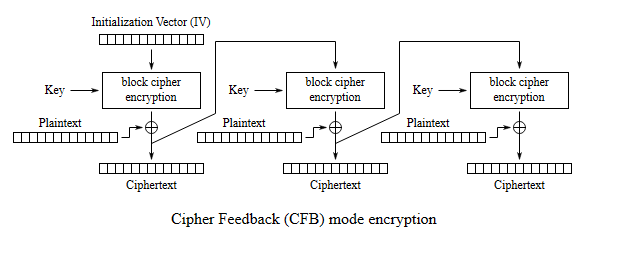
\includegraphics[height=\textheight,width=\textwidth,keepaspectratio]
    {figures/CFB_encryption.png}
    \caption{Cipher Feedback (CFB) mode encryption~\cite{cipher_mode_wiki}.}\label{fig:cfb_enc}
\end{figure}

\begin{figure}
    \centering
    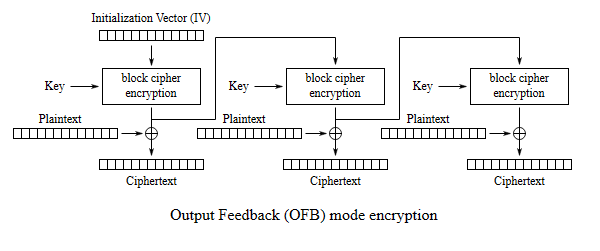
\includegraphics[height=\textheight,width=\textwidth,keepaspectratio]
    {figures/OFB_encryption.png}
    \caption{Output Feedback (OFB) mode encryption~\cite{cipher_mode_wiki}.}\label{fig:ofb_enc}
\end{figure}

\subsection{Data added during padding}
%
\begin{lstlisting}[language=Bash, caption=Files inside the
    the task4 folder]
[02/08/23]seed@VM:~/.../task4$ ls
10byte.txt  5byte.txt       cbc  ecb  password.txt
16byte.txt  auto_script.sh  cfb  ofb
\end{lstlisting}

\begin{lstlisting}[language=Bash, caption=Using {\fontfamily{qcr}\selectfont
    auto\_script.sh} with the CBC mode., label={lst:auto_script_example}]
$ ./auto_script.sh cbc
\end{lstlisting}

\begin{lstlisting}[language=Bash, caption=Automating script for discovering
    what was added to the padding during encryption/decryption ({\fontfamily{qcr}
    \selectfont auto\_script.sh}), label={lst:padding_script}]
#! /bin/bash
mode=$1

cp *.txt $mode
cd $mode
arr=($(ls *byte.txt))
for i in "${arr[@]}"
do
    # Encryption
    openssl enc -e -aes-128-$mode -kfile password.txt -pbkdf2 -in ${i} -out ${i}.enc
    # Decryption
    openssl enc -d -aes-128-$mode -kfile password.txt -pbkdf2 --nopad -in ${i}.enc -out ${i}.dec

done
\end{lstlisting}

As we used AES-128 block cipher in this case, the block size is 128 bits or 16 bytes.
Note that the number 128 in AES-128 indicates the key size. The block size of plaintext
must be a multiple of 16 in bytes. OpenSSL uses PKCS padding method by default. PKCS
states the following rules~\cite{pkcs_padding}:
\begin{enumerate}
    \item Padding bytes must be added to the plaintext before it is encrypted.
    \item The value of each padding byte equal the number of bytes needed to be added.
    For example, if the plaintext is 12-byte long, the number of bytes needed to be added
    is 4 (the block size in AES is 16 bytes). Hence, the value of each padding byte is 0x04.
    \item The total number of padding bytes is at least one, and is the number that is
    required to raise the data length up to a multiple of block size.
\end{enumerate}

In this work, in order to illustrate what OpenSSL adds during encryption/decryption, we
did the following steps:
\begin{enumerate}
    \item Create three files {\fontfamily{qcr}\selectfont 5byte.txt, 10byte.txt,
    16byte.txt} that are 5-byte, 10-byte, and 16-byte long respectively.
    \item Create separate folders for each cipher mode ``ecb'', ``cbc'', ``ofb'',
    and ``cfb''.
    \item Create {\fontfamily{qcr}\selectfont password.txt} storing the password
    for generating keys.
    \item Run {\fontfamily{qcr}\selectfont auto\_script.sh} (\autoref{lst:padding_script}).
    This script hepls us automate the process of encrypting and decrypting target files.
    Please look at \autoref{lst:auto_script_example} to know how to run the script.
    \item Investigate the padding bytes of each file by {\fontfamily{qcr}
    \selectfont xxd} command.
\end{enumerate}

In the case of ECB (\autoref{fig:padding_ecb}) and CBC (\autoref{fig:padding_cbc}),
the value of each padding byte and the number of adding bytes are the number of bytes
required to fulfill the block of ciphertext such that it is a multiple of the block size
, 16 bytes in AES. For example, in {\fontfamily{qcr}\selectfont 5byte.txt}, a file that
is 5-byte long, it needs more 16-5=11 bytes to fulfill the size of block. Hence, 11 more
bytes were added, and the value of each adding byte was 0x0b in hexadecimal, or 11 in decimal.
In the case of {\fontfamily{qcr}\selectfont 16byte.txt}, its lenght is already a multiple
of 16, 16-byte long. However, according to PKCS's rule, the total number of padding bytes
must be at least one. Thus, there were 16 bytes (a whole block) added, and the value of
each byte was 0x10 in hexadecimal, or 16 in decimal.

In the case of OFB (\autoref{fig:padding_ofb}) and CFB (\autoref{fig:padding_cfb}), there
were not any bytes added since these modes do not require padding.

% Figures of showing hexadecimal content of files
\begin{figure}
    \centering
    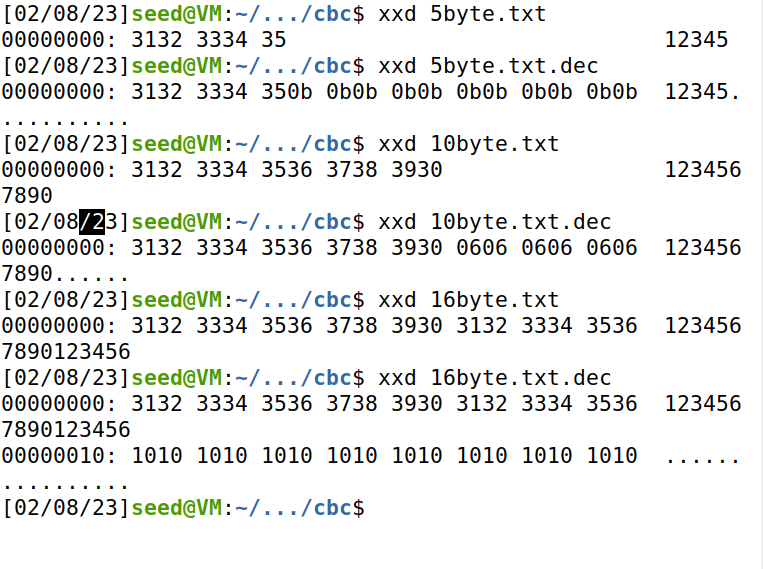
\includegraphics[height=\textheight,width=\textwidth,keepaspectratio]
    {figures/padding_cbc.png}
    \caption{Original and decrypted files using CBC mode.}\label{fig:padding_cbc}
\end{figure}

\begin{figure}
    \centering
    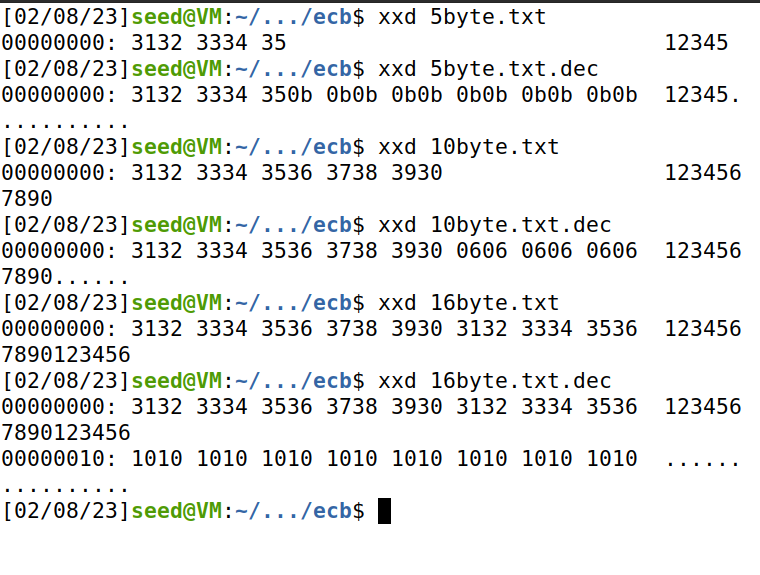
\includegraphics[height=\textheight,width=\textwidth,keepaspectratio]
    {figures/padding_ecb.png}
    \caption{Original and decrypted files using ECB mode.}\label{fig:padding_ecb}
\end{figure}

\begin{figure}
    \centering
    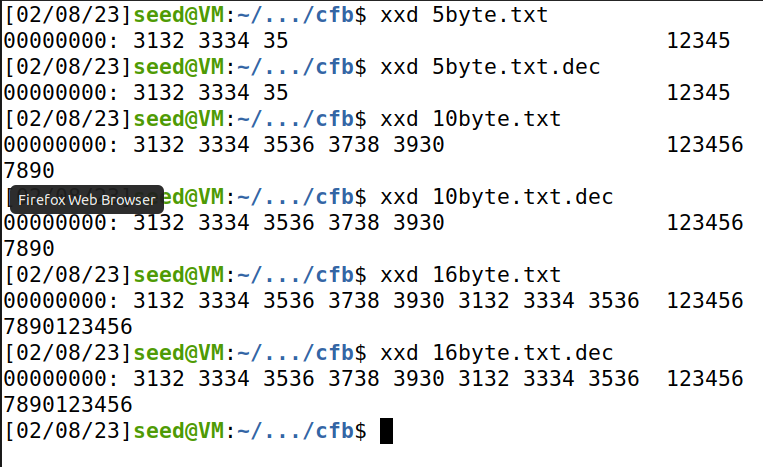
\includegraphics[height=\textheight,width=\textwidth,keepaspectratio]
    {figures/padding_cfb.png}
    \caption{Original and decrypted files using CFB mode.}\label{fig:padding_cfb}
\end{figure}

\begin{figure}
    \centering
    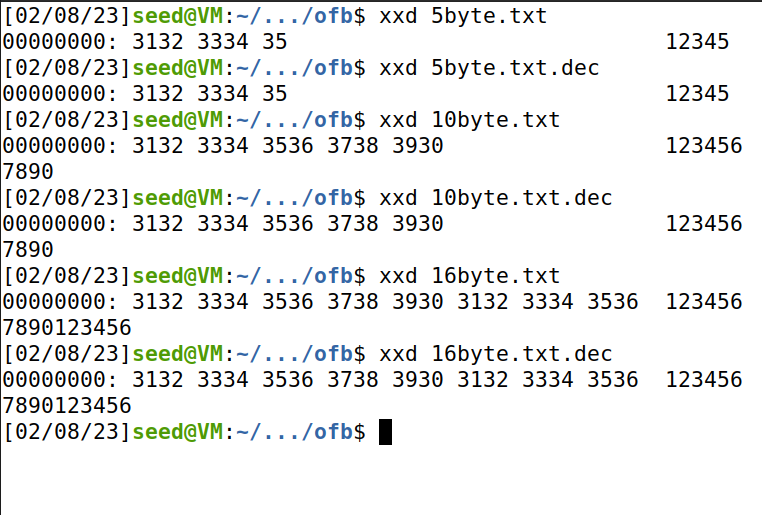
\includegraphics[height=\textheight,width=\textwidth,keepaspectratio]
    {figures/padding_ofb.png}
    \caption{Original and decrypted files using OFB mode.}\label{fig:padding_ofb}
\end{figure}